\documentclass{article}
\usepackage[utf8]{inputenc}
\usepackage{apacite}
\usepackage{graphicx}   
\graphicspath{{figures/}}

\title{Why are we still building AR Piano Teaching Systems? A Review of Augmented Reality Piano Teaching Systems}
\author{Jordan Aiko Deja}
\begin{abstract}
     %Humans have been using and learning the piano for over 3 centuries. In recent years, innovations that support learning music instruments including the piano have been introduced. Many reviews have been done on prototypes that enhance learning experiences with Augmented Reality (AR). While some of these reviews explored a wide range of AR prototypes, a thorough review of systems supporting piano have yet to be done. In this paper, we first explore AR piano prototypes using a systematic search. Second, we review the different innovations in these prototypes and organise them into contribution categories. Third, we discuss the impact of these contributions and provide recommendations on 
     Humans have been using and learning the piano for over 3 centuries. In the last 15 years, several Augmented Reality (AR) piano prototypes that support learning have been introduced. Why are we still building these prototypes? What do these systems lack? In this paper, we present a systematic review of AR piano prototypes developed within the recent years. We review the different innovations they present and organise them into contribution categories. We will then discuss the impact of these contributions and recommend directions for future work towards designing better AR piano prototypes. 
    % Augmented Reality (AR) piano teaching systems …. Many AR piano teaching systems are available for .. while many research prototypes have tried to .. The development of these tools was based on knowledge drawn from fields of computer graphics, ubiquitous and mobile computing, human-computer interaction and cognitive psychology. 
     
\end{abstract}
\date{July 2020}

\begin{document}

\maketitle


\nocite{*}



\section{Introduction}
Survey of AR piano teaching systems and prototypes
Discussion on how these prototypes were evaluated and how the research focus has changed over the last 15 years
Overview of what technological contributions were made and future steps 

.. This paper focuses on X prototypes categorized and sorted by .. These sections describe prototypes that addressed problems in (enumerate). In each section, prototypes are grouped in subsection compared by its .. They are also listed in chronological order to show the course of development. Each subsection ends with a short discussion about .. This paper concludes with an overview discussion and a conclusion about ..


\section{Background}
Augmented Reality
Augmented reality piano teaching systems
Design Factors affecting augmented reality piano teaching systems (hardware, software, content)



\begin{figure}
    \centering
    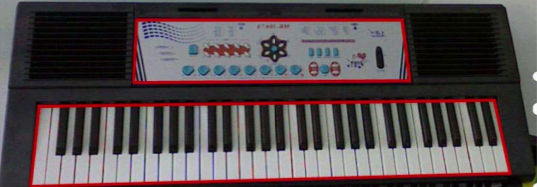
\includegraphics[width=15cm]{figures/pianomarker.png}
    \caption{Piano Augmented Reality marker}
    \label{fig:pianomarker}
\end{figure}



\section{Method}
Meta-analysis (Search for prototypes, Inclusion criteria, data gathering)
Qualitative Analysis (search for prototype, inclusion criteria, data gathering)
How did you do the review? What were the sources and keywords used? What was the qualifying criteria? 
How did you organize the prototypes? By what categories? How is the rest of the document then sorted based on these categories? 



\begin{figure}
    \centering
    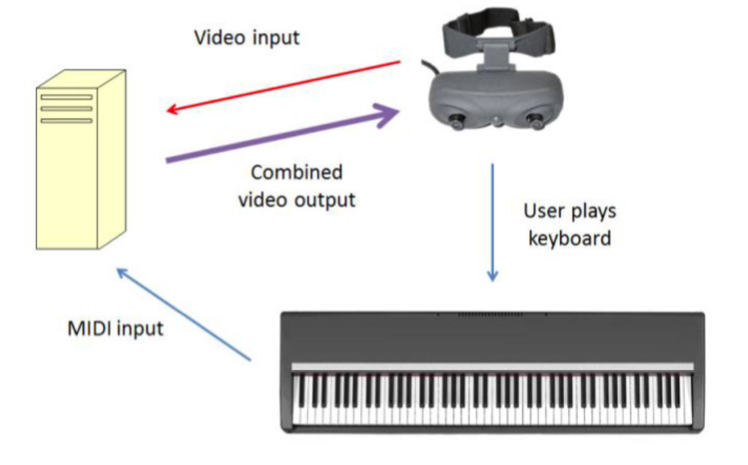
\includegraphics[width=10cm]{figures/headmountedpiano1.png}
    \caption{Architecture of the Head Mounted Piano by cite! }
    \label{fig:pianoheadmountedarch}
\end{figure}

\begin{figure}
    \centering
    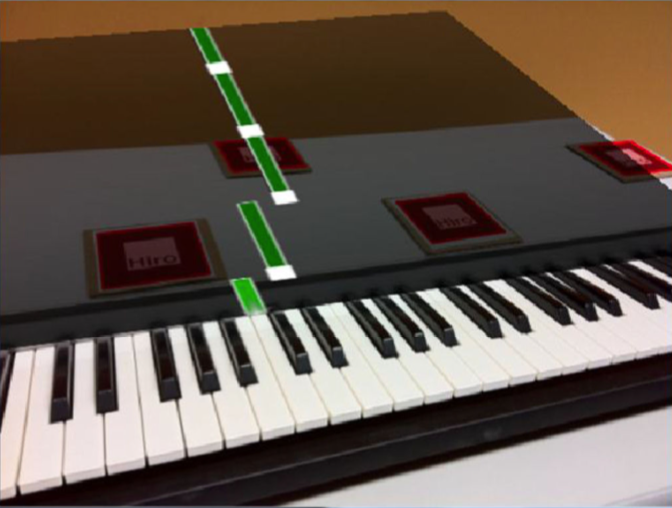
\includegraphics[width=10cm]{figures/headmountedview.png}
    \caption{View from the Head Mounted Piano AR  }
    \label{fig:View from the HeadMounted}
\end{figure}


\section{Affordances of AR piano teaching systems}


\section{Design Strategies of AR piano teaching systems}

\begin{figure}
    \centering
    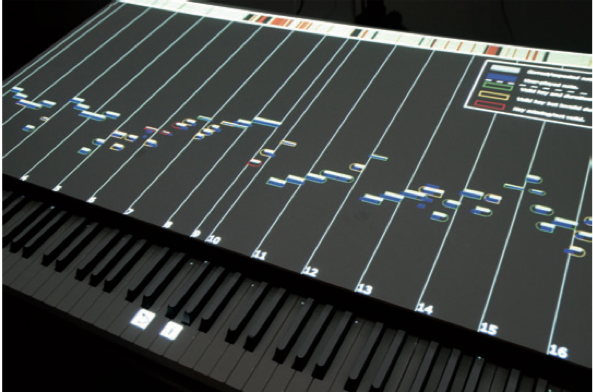
\includegraphics[width=10cm]{figures/piano}
    \caption{View of the Detailed Screen of P.I.A.N.O.› }
    \label{fig:View from the HeadMounted}
\end{figure}



\section{Visualisations}
Section discussing prototypes whose main contributions focused on visualizations, overlaying graphics, rendering and optimization etc


\section{Agents and Tutors}
Section discussing prototype whose main contributions focused on virtual agents/tutors 

\section{Learning Modes}
Section discussing prototype whose contributions focused on learning modes, emphasis on pedagogy and other learner-centric modes

\section{Evaluation Techniques}
done by studies on AR piano teaching systems (hypothesis based on cognition, realistic annotations etc)

\section{Discussion and Future Directions}

\section{Tables and Figures}
Table of papers divided by number of participants and whether authors were from academia or industry
Figure of number of participants per study by years, size of each bubble is relative to sizes of other bubbles and based on number of participants in a study. Sort per category 
Figure/Table of all described prototypes with year, by type with number of participants, short study description, number of citations and if authors are from academia or industry
Table of Studies evaluating learner performance with effect sizes (content, sample, control group, treatment, effect, size)
Table of Studies evaluating learner performance 
Figure of number of AR piano teaching system publications until june 2020
Table of AR piano teaching systems with corresponding devices 
Table of AR piano teaching systems showing summary of survey questionnaires


% overview of audio augmented reality
% classical works in audio augmented reality
% visualizations in audio
% audio and lighting effects in performance media
% usability studies involving audio augmented reality
% novel works and audio ar on inclusive music (for def or pwd)




% music features and visualization

% taxonomy of AR and music 

% music decorates space by andre
% using visualization 




\bibliographystyle{apacite}
\bibliography{references}

\end{document}
